%%%%%%%%%%%%%%%%%%%%%%%%%%%%%%%%%%%%%%%%%%%%%%%%%%%%%%%%%%%%%%%%%%% 
%                                                                 %
%                            CHAPTER                              %
%                                                                 %
%%%%%%%%%%%%%%%%%%%%%%%%%%%%%%%%%%%%%%%%%%%%%%%%%%%%%%%%%%%%%%%%%%% 

\chapter{Inleiding}

\section{Situering}
Sociale media is zo goed als niet meer weg te denken uit het huidige moderne
leven. Over de jaren heen zijn er dan ook verschillende definities gegeven.
\citeauthor{PhilipsAndParks} definiëren sociale media als de infrastructuur en
tools om content te maken en te verspreiden\cite{PhilipsAndParks}. Deze
definitie is erg ruim, en vertakt zich dus in heel wat facetten, waaronder
sociale netwerken, media sharing networks,\ldots Maar ook de fitnesstrackers.
Deze opkomst van nieuwe media brengen echter ook vaak onbedoelde maar
significante privacy bezorgdheden met zich mee.

De focus in deze dissertatie ligt op privacy binnen fitnesstrackers, meer
specifiek platformen die gps-locaties gebruiken, zoals Strava, Nike Run Club,
etc. Dit zijn platformen waar sportactiviteiten zoals lopen, fietsen,
wandelen,\ldots kunnen worden gedeeld met andere personen. Het algemene concept
is hierbij dat wanneer je een sportactiviteit uitvoert, je deze voor je volgers
en vrienden beschikbaar maakt. De sportactiviteit zal dan natuurlijk ook
bepaalde gegevens bevatten die zichtbaar zijn voor die volgers, zoals
tijdstippen, hartslagen, bewegingstijd, en vaak ook
gps-locaties~\ref{fig:activityExample}. Vele van deze gegevens hebben direct of
indirect een negatieve impact op de privacy van de user. Deze negatieve
gevolgen komen dan vooral in de vorm van het onbedoeld vrijgeven gevoelige
locaties. Dit kan gaan over woonplaatsen, wat kan leiden tot o.a.\ stalking.
Alsook locaties waar sportmateriaal wordt opgeborgen. Er zijn gevallen bekend
van fietsdieven die Strava gebruiken om fietsen te kunnen
lokaliseren\cite{Sportapp72:online}\cite{Cyclistw89:online}. Grootschaligere
voorbeelden die zeker het vermelden waard zijn de gevallen waarbij geheime
militaire basissen ontdekt worden door het bestuderen van de heatmap.
\begin{figure}
    \centering
    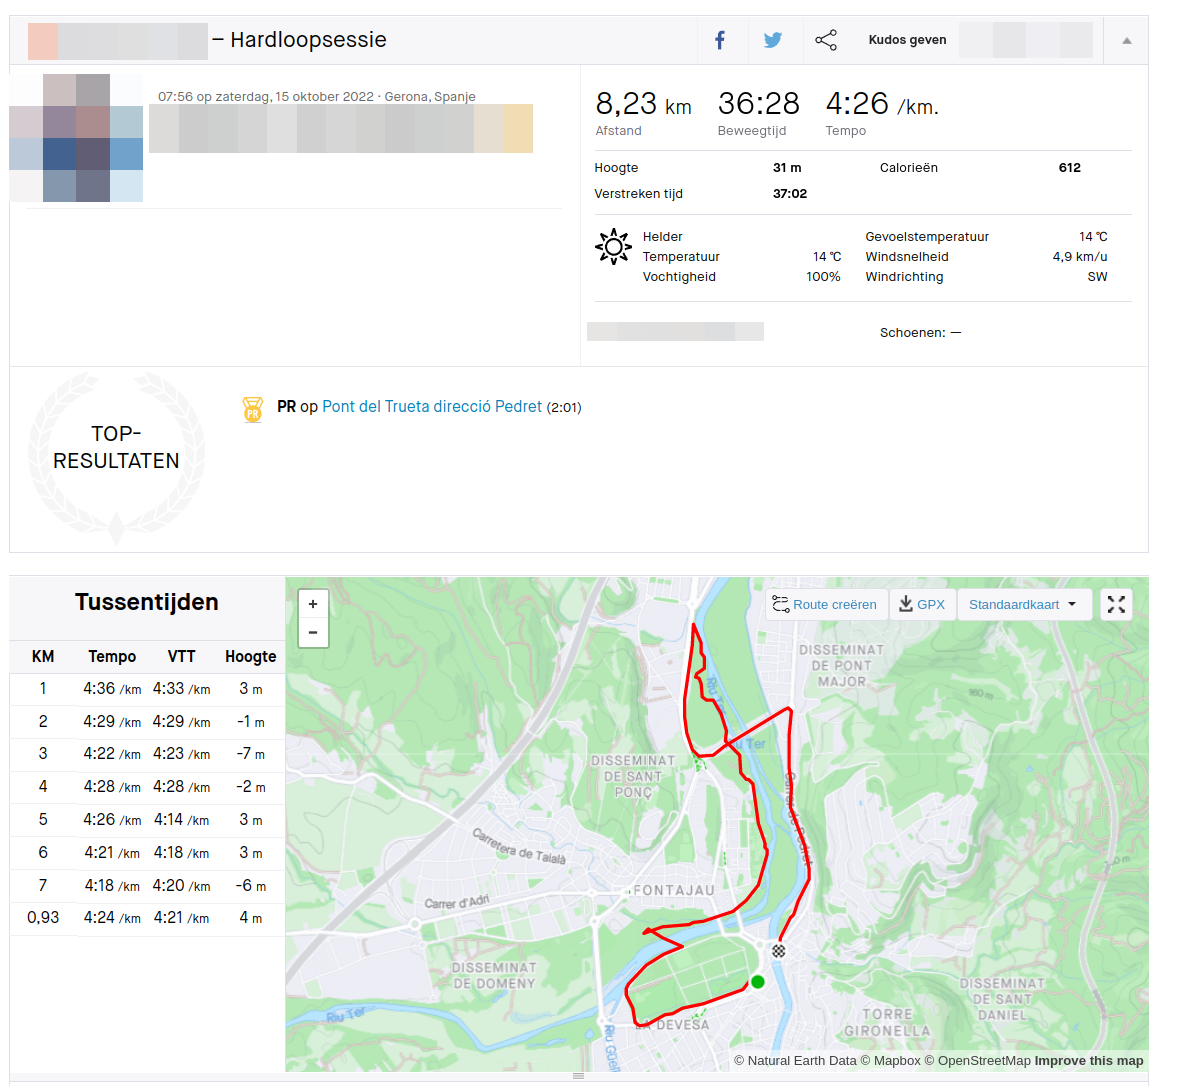
\includegraphics[width=0.5\linewidth]{fig/VoorbeeldActiviteit_Cropped.png}
    \caption{Voorbeeldactiviteit Strava}\label{fig:activityExample}
\end{figure}

Deze platformen implementeren elk manieren om de privacy van de users te
verbeteren. Hiervoor zijn verschillende manieren mogelijk. De simpelste is
misschien wel de mogelijkheid om activiteiten te verbergen voor een selectie
van personen (bv.\ enkel weergeven voor je volgers). Zo kunnen enkel de mensen
die de gebruiker expliciet toelaat activiteiten bekijken. Een complexere
alternatief is het gebruik van \textit{endpoint privacy zones} (EPZ). Hierbij
wordt de weergegeven route voor de persoon die meekijkt gedeeltelijk verborgen.
Er wordt als het ware een deel van de route afgekapt, en het eind- en startpunt
worden verschoven. Het begin- en eind-deel van de route wordt dus onzichtbaar
voor de andere gebruikers. Het valt op dat de ontwikkelaars van de platformen
erg bewust zijn van de mogelijke gevaren. Echter is er een afweging te maken
bij de implementatie tussen de bruikbaarheid van het platform, en de privacy
van de eindgebruiker. Hoe meer info wordt vrijgegeven, hoe groter de kans om
mogelijk schadelijke private info wordt meegegeven. Aan de andere kant, bij het
weglaten van informatie gaat de gebruiksvriendelijkheid en de aanwezigheid van
nuttige info van het platform serieus achteruit gaat.

\section{Doelstelling}
Het doel van deze scriptie is om private locaties (verborgen start- en
eindlocaties) van een activiteiten te achterhalen, ondanks het gebruik van de
EPZ~\ref{EPZ} als privacy beveiligingsmechanisme. In het verleden werden enkele
manieren beschreven om a.d.h.v.\ andere metadata zoals hoogtedata en afstanden
de EPZ te omzeilen
(\textit{\citeauthor{Dhondt_Pochat_Voulimeneas_Joosen_Volckaert_2022},
    \citeauthor{Verdonck_2022}}). Gedurende deze thesis wordt meer in detail gegaan
op het gebruik van snelheidsdata. Als basis voor deze aanval wordt de
inferentie aanval op de EPZ
van~\citeauthor{Dhondt_Pochat_Voulimeneas_Joosen_Volckaert_2022} genomen. Er
wordt dan onderzocht of deze aanval nog succesvol kan worden uitgevoerd bij het
weglaten van bepaalde gegevens, en dus door het gebruik van andere gegevens,
voornamelijk snelheid.

Om deze doelstelling te bekomen zal eerst een analyse op de afwijkingen van
tussen de berekende afstanden nodig om de inferentie aanval uit te voeren, en
de waarden afgeleid volgens de berekeningen
van~\citeauthor{Dhondt_Pochat_Voulimeneas_Joosen_Volckaert_2022}. Er zal een
analyse gebeuren over de alle users. Er zal ook een studie gebeuren van de
effectiviteit van deze aanval op basis van de nieuw bekomen afstanden.

De doelstellingen zijn in eerste instantie vooral vanuit het oogpunt van een
aanvaller, een user met slechte bedoelingen. Echter zal naar het einde toe ook
gereflecteerd worden over de gevallen waarin de aanval effectief blijft,
bijvoorbeeld onder welke afrondingen. Bijgevolg kunnen hieruit enkele mogelijke
countermeasures worden afgeleid, die dus zullen aangeven welke manieren
fitnesstrackers zichzelf zouden kunnen toepassen om zichzelf te wapenen tegen
de aanval die hier beschreven werd.